
\chapter*{CAPITULO I TITULO DEL CAPITULO}

%\vspace{-0.7cm}
\addcontentsline{toc}{chapter}{CAPITULO I TITULO DEL CAPITULO}

%------------------------------------------------------------------------- 
Esta plantilla se hizo con la finalidad de poder agilizar la realización del documento de tesis, facilitando un formato definido y listo para usar. A lo largo del documento encontrará comentarios y explicaciones de como usar las diferentes "herramientas" que entrega Latex.

% Titulo de ejemplo 1.1
\section{1.1 Titulo de ejemplo 1}

% Poner un texto en negritas con \textbf{TEXTO}
% Poner un texto en cursiva con \textit{TEXTO}
% Poner un texto en negritas y cursiva con \textbf{\textir{TEXTO}}
Lorem ipsum dolor sit amet, \textbf{consectetur adipiscing elit, sed do eiusmod tempor incididunt ut labore et dolore magna aliqua}. Ut enim ad minim veniam, quis nostrud exercitation ullamco laboris nisi ut aliquip ex ea commodo consequat. Duis aute irure dolor in reprehenderit in voluptate velit esse cillum dolore eu fugiat nulla pariatur. Excepteur sint occaecat cupidatat non proident, sunt in culpa qui officia deserunt mollit anim id est laborum.
% Para citar solo debe poner \cite{nombre cita}
\textit{Lorem ipsum dolor sit amet, consectetur adipiscing elit, sed do eiusmod tempor incididunt ut labore et dolore magna aliqua}. Ut enim ad minim veniam, quis nostrud exercitation ullamco laboris nisi ut aliquip ex ea commodo consequat. \textbf{\textit{Duis aute irure dolor in reprehenderit in voluptate velit esse cillum dolore eu fugiat nulla pariatur}}. Excepteur sint occaecat cupidatat non proident, sunt in culpa qui officia deserunt mollit anim id est laborum.

% Modificar "\newcommand{\descripcion}{....} para describir el contenido de la tabla.
% Modificar la fuente según corresponda. 
\begin{table}[ht]
    \centering
    \newcommand{\descripcion}{Descripción de la tabla.}
    \caption*{Tabla \arabic{cap1}.\arabic{tabla}: \descripcion}
    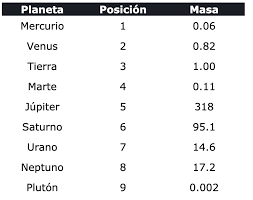
\includegraphics{figuras/tabla-ejemplo.png}\\
    {\textit{\small Fuente: } \textit{\small Autores por apellido (año). Titulo del documento de donde se copio la figura.}}
    \label{Tabla: Tabla ejemplo}
    \addcontentsline{lot}{table}{Tabla \arabic{cap1}.\arabic{tabla}: \descripcion}
    \addtocounter{tabla}{1}
\end{table}
% \label nos permite referenciar la tabla/figura en otra parte del documento.

% Subtitulo de ejemplo 1.1.1
\subsection{1.1.1 Subtitulo de ejemplo 1}

Lorem ipsum dolor sit amet, consectetur adipiscing elit, sed do eiusmod tempor incididunt ut labore et dolore magna aliqua. Ut enim ad minim veniam, quis nostrud exercitation ullamco laboris nisi ut aliquip ex ea commodo consequat. Duis aute irure dolor in reprehenderit in voluptate velit esse cillum dolore eu fugiat nulla pariatur. Excepteur sint occaecat cupidatat non proident, sunt in culpa qui officia deserunt mollit anim id est laborum.

% Subtitulo de ejemplo 1.1.2
\subsection{1.1.2 Subtitulo de ejemplo 2}

Lorem ipsum dolor sit amet, consectetur adipiscing elit, sed do eiusmod tempor incididunt ut labore et dolore magna aliqua. Ut enim ad minim veniam, quis nostrud exercitation ullamco laboris nisi ut aliquip ex ea commodo consequat. Duis aute irure dolor in reprehenderit in voluptate velit esse cillum dolore eu fugiat nulla pariatur. Excepteur sint occaecat cupidatat non proident, sunt in culpa qui officia deserunt mollit anim id est laborum.

% Subtitulo de ejemplo 1.1.3
\subsection{1.1.3 Subtitulo de ejemplo 3}

Lorem ipsum dolor sit amet, consectetur adipiscing elit, sed do eiusmod tempor incididunt ut labore et dolore magna aliqua. Ut enim ad minim veniam, quis nostrud exercitation ullamco laboris nisi ut aliquip ex ea commodo consequat. Duis aute irure dolor in reprehenderit in voluptate velit esse cillum dolore eu fugiat nulla pariatur. Excepteur sint occaecat cupidatat non proident, sunt in culpa qui officia deserunt mollit anim id est laborum.

%-------------------------------------------------------------------------
% Titulo de ejemplo 1.2
\section{1.2 Agregar formulas matemáticas}

Para agregar formulas matematicas en el texto se deben escribir entre "$ $", aquí podemos ver un ejemplo: 
El área de un círculo de radio r se puede calcular mediante la fórmula $A = \pi r^2$.
Fórmula para calcular la suma de los primeros n números enteros:  
\begin{equation}
    \sum_{i=1}^{n} i = \frac{n(n+1)}{2}
\end{equation}

Fórmula cuadrática:
\begin{equation}
    x = \frac{-b \pm \sqrt{b^2 - 4ac}}{2a}
\end{equation}

Teorema de Pitágoras:
\begin{equation}
    c = \sqrt{a^2 + b^2}
\end{equation}

Función exponencial:
\begin{equation}
    f(x) = e^x
\end{equation}

Fórmula de Euler:
\begin{equation}
    e^{i\theta} = \cos\theta + i\sin\theta
\end{equation}

Ley de Ohm:
\begin{equation}
    V = IR
\end{equation}


%-------------------------------------------------------------------------
% Titulo de ejemplo 1.3
\section{1.3 Titulo de ejemplo 3}

Lorem ipsum dolor sit amet, consectetur adipiscing elit, sed do eiusmod tempor incididunt ut labore et dolore magna aliqua. Ut enim ad minim veniam, quis nostrud exercitation ullamco laboris nisi ut aliquip ex ea commodo consequat. Duis aute irure dolor in reprehenderit in voluptate velit esse cillum dolore eu fugiat nulla pariatur. Excepteur sint occaecat cupidatat non proident, sunt in culpa qui officia deserunt mollit anim id est laborum.

% Modificar "\newcommand{\descripcion}{....} para describir el contenido de la tabla.
% Modificar la fuente según corresponda. 
% Puede ajustar el tamaño de la figura modificando el parametro "scale", ej: 0.5 (1 corresponde al tamaño original)
\begin{figure}[H]
    \centering
    \newcommand{\descripcion}{Descripción de la figura.}
    \caption*{Figura \arabic{cap1}.\arabic{figura}: \descripcion}
    
\includegraphics[scale=0.2]{figuras/dpto-industrias-usach.jpg}\\
    {\textit{\small Fuente: } \textit{\small Autores por apellido (año). Titulo del documento de donde se copio la figura.}}
    \label{fig:Dpto_Industrias}
    \addcontentsline{lof}{figure}{Figura \arabic{cap1}.\arabic{figura}: \descripcion}
    \addtocounter{figura}{1}
\end{figure}
% \label nos permite referenciar la tabla/figura en otra parte del documento.

%------------------------------------------------------------------------
% Titulo de ejemplo 1.4
\section{1.4 Listando información}

Para listar información se presentan 2 formas de hacerlo; de forma ordenada y de forma desordenada. A continuación se presenta en más detalle cada una de ellas

% Subtitulo de ejemplo 1.4.1
\subsection{1.4.1 Listar en forma ordenada}

A continuación un ejemplo de como listar información en forma ordenada:
\begin{enumerate}
    \item Ejemplo 1
    \item Ejemplo 2
    \item Ejemplo 3
    \item Ejemplo 4
\end{enumerate}

% Subtitulo de ejemplo 1.4.2
\subsection{1.4.2 Listar en forma desordenada}

A continuación un ejemplo de como listar información en forma desordenada:
\begin{itemize}
    \item Ejemplo 1
    \item Ejemplo 2
    \item Ejemplo 3
    \item Ejemplo 4
\end{itemize}